\section{Photonic Lantern Information Determination}

	This section contains information about the euclidean distances comparison between the different spaces along the optical pathway.
	
	\subsection{Purpose}
		
		The purpose of this project is to determine the relationship between the different spaces along the optical pathway to check of the information is conserved. If two PSFs are similar or have a small euclidean distance between them, how similar will the output fluxes be?
		
		To do this we select pairs of points from our datasets and measure the euclidean distances between them plotting the relationships in a scatter plot.
		
		
	\subsection{The data}
		
		There are 4 different types of datasets:
		\begin{itemize}
			\item Zernike coefficients
			\item PSF
			\item LP coefficients
			\item Photonic Lantern Output fluxes
		\end{itemize}
		
		The paths to the datasets can be found in the file \href{https://github.com/Dacarpe03/PLImageReconstruction/blob/main/Utils/psf_constants.py}{psf\_constants.py}.\\
		
		In this case the PSFs are generated from Zernike coefficients instead of atmospheric aberrations so the function to generate them is \filename{generate\_zernike\_psf\_complex\_fields} which can be found in the file  \href{https://github.com/Dacarpe03/PLImageReconstruction/blob/main/Utils/data_utils.py}{data\_utils.py}.\\
		
	\subsection{Results}
		
		\begin{figure*}[ht!]
			\centering
			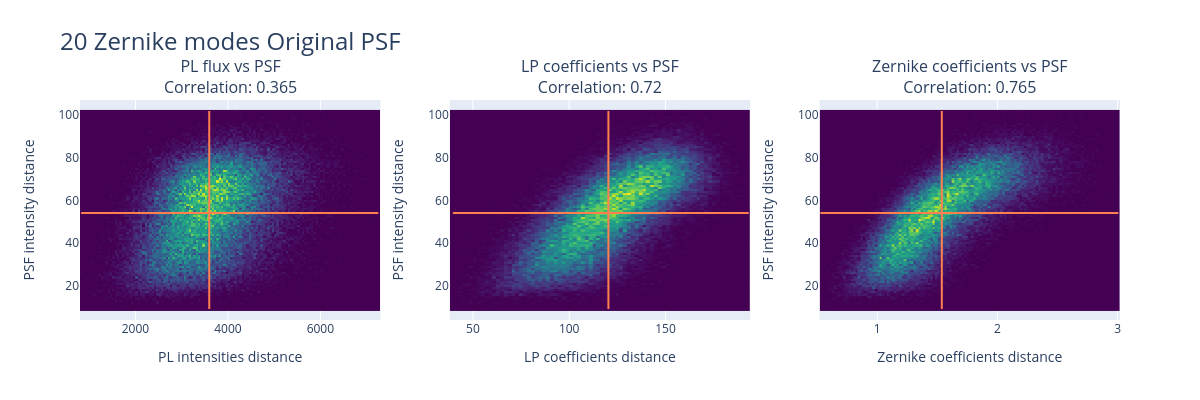
\includegraphics[width=0.9\textwidth]{pid-20mOriginalpsfdistances.png}
		\end{figure*}
		\FloatBarrier
		
		These plots are done as follows:
		\begin{enumerate}
			\item Chose a set of pairs of points. One point is a set of Zernike Coefficients, the PSF intensity they define, the LP coefficients from the overlap integral of the PSF with the LP modes and the output fluxes obtained after multiplying the transfer matrix with the LP coefficients.
			\item Compute the euclidean distances between:
				\begin{itemize}
					\item Zernike Coefficients of each point
					\item Flattened PSF intensity matrix
					\item Flattened complex LP coefficients
					\item Output flux intensities of the PSF
				\end{itemize}
			\item The coordinates of each point in the above plot represent the euclidean distance in two different optical pathway spaces. (In the first on the left the y coordinate represent the distance between a pair of points in the PSF intensities space and the x coordinate the distance between the same pair of points in the Photonic Lantern fluxes space).
		\end{enumerate}
		
		The results tell us that similarity between PSF imply similarity between PL fluxes but not viceversa.
		
	\subsection{Code}
		\begin{itemize}
			\item To measure the euclidean distances use the notebook \href{https://github.com/Dacarpe03/PLImageReconstruction/blob/main/PSFReconstruction/DataNotebooks/PLInformationDetermination.ipynb}{PLInformationDetermination.ipynb}
			\item To plot the cloud of euclidean distances use the notebook \href{https://github.com/Dacarpe03/PLImageReconstruction/blob/main/PSFReconstruction/Plots/LowOrderZernikePLInformationPlots.ipynb}{LowOrderZernikePLInformationPlots.ipynb} for zernike generated datasets or \href{https://github.com/Dacarpe03/PLImageReconstruction/blob/main/PSFReconstruction/Plots/PLInformationPlots.ipynb}{PLInformationPlots.ipynb}
		\end{itemize}
		
	\subsection{Detailed results}
	
		For a detailed report on the datasets, results and plots see Part III from \filename{appendix.pdf.pdf}.
		